\documentclass{article}
\usepackage[utf8]{inputenc}
\usepackage{graphicx} % For including images
\usepackage{amsmath} % For mathematical symbols and equations
\usepackage{hyperref} % For hyperlinks
\usepackage{xcolor} % For customizing colors
\usepackage{subcaption}

\hypersetup{
    colorlinks=true,
    linkcolor=blue, % Set the color of internal links
    urlcolor=blue, % Set the color of external links
    citecolor=blue % Set the color of citation links
}


\title{Estimating the Sim2Real Gap for Camera Simulation Using Existing Visual Odometry Algorithms}
\author{Sriram Ashokumar \and Huzaifa Unjhawala}
\date{\today}

\begin{document}

\maketitle

\section{Introduction}
\subsection{Overview}
The sim-to-real gap poses a challenge for existing visual odometry (VO) algorithms. These algorithms often require extensive fine-tuning when deployed in real-world scenarios, demanding considerable resources for effective implementation. To address this issue, there is a \textbf{growing emphasis on tuning and testing VO algorithms in simulation environments}, with the goal of deploying them in reality with minimal to no additional fine-tuning. However, the effectiveness of these algorithms is further tested when they encounter out-of-distribution environments in reality, highlighting the need for robust and adaptable VO solutions that can seamlessly transition from simulated to real-world settings.  

In this project, we aim to quantify the sim2real gap of a simulator (\href{https://projectchrono.org/}{Project Chrono}) using a testing platform (\href{https://github.com/uwsbel/autonomy-research-testbed}{Autonomy Research Testbed}) developed in-house and an existing VO algorithm.

\subsection{Sim2Real Quantification Approach}
We plan to use a ``judge'' based approach for the quantification of the sim2real gap of the sensors used in the Visual Odometry algorithm. Herein, the ``judge'' is the chosen VO/VIO algorithm. We call this algorithm a ``judge'' because the quality of the simulated sensors and the simulation environment is ``judged'' based on the performance of the VO/VIO algorithm. For good quality simulated sensors and sensor environment, we expect the performance of the ``judge'' to be the same irrespective of whether it listens to simulated sensor data in the simulation environment or real sensor data in the real data. Specifically, we expect the \textbf{localization errors in simulation to match those in reality}. If the VO/VIO algorithm has a high error in simulation, we would like for it to have a high error in reality and vice-versa. This would mean that the simulated sensors and the environment are a good representation for reality for the development of VO/VIO algorithm. Although we have not nailed down the exact mathematical metric we will use, or that we will reach a stage where we have all the data required to evaluate this metric, this will be the overall long-term approach.

\section{Proposed Plan of Action}

\subsection{Literature Review}
Our initial step involves conducting a literature review focusing on recent advancements in VO and visual-inertial odometry (VIO) algorithms. This review aims to identify algorithms that demonstrate robust performance across standard datasets, such as EuROC and KITTI, and to assess their ease of use, installation feasibility due to dependencies, and overall performance.

\subsection{Algorithm Selection and Evaluation}
From the literature, we planned to select four VO/VIO algorithms for a deeper evaluation, considering their ease of use, installation requirements, and performance metrics. The selection criteria was to primarily revolve around their demonstrated effectiveness on benchmark datasets.

\subsection{Simulation and Real-World Testing}
Upon selecting a suitable VO/VIO algorithm, we planned to create a simulation environment using Project Chrono and set up a real vehicle equipped with necessary sensors. Both environments would utilize a ROS2 stack for integrating the chosen VO/VIO algorithm, enabling a comparative analysis of localization errors in simulation versus reality.

\section{Progress Made So Far}
We have made progress on several fronts. We describe here the four primary fronts and the progress made in each.
\subsection{Picking a VO/VIO Algorithm}
To determine which VO/VIO algorithm to use, we first performed a literature review of existing algorithms. We mainly explored recent advancements in visual odometry (VO) and visual-inertial odometry (VIO), focusing on benchmark performance, underlying methodologies, strengths and weaknesses, computational requirements, and sensor needs. We initially narrowed it down to 10 papers by doing a quick read. These papers include:


\begin{enumerate}
    \item DROID-SLAM: Deep Visual SLAM for Monocular, Stereo, and RGB-D Cameras (2021)
    \item RD-VIO: Robust Visual-Inertial Odometry for Mobile Augmented Reality in Dynamic Environments (2023)
    \item ORB-SLAM3: An Accurate Open-Source Library for Visual, Visual-Inertial, and Multi-Map SLAM (2021)
    \item OpenVSLAM: A Versatile Visual SLAM Framework (2019)
    \item VOLDOR: Visual Odometry from Log-logistic Dense Optical Flow Residuals (2020)
    \item TartanVO: A Generalizable Learning-based VO (2020)
    \item UnDeepVO: Monocular Visual Odometry through Unsupervised Deep Learning (2018)
    \item AirVO: An Illumination-Robust Point-Line Visual Odometry (2023)
    \item Beyond Tracking: Selecting Memory and Refining Poses for Deep Visual Odometry (2019)
    \item VRVO: Towards Scale Consistent Monocular Visual Odometry by Learning from the Virtual World (2022).
\end{enumerate}
\subsubsection*{Performance on standard datasets}
All of these papers demonstrate strong performance on standard datasets like KITTI, EuRoC MAV, and TUM-RGBD. DROID-SLAM boasts impressive accuracy improvements over prior work, while RD-VIO excels in dynamic environments. ORB-SLAM3 exhibits high accuracy and robustness across various sensor configurations. OpenVSLAM, VOLDOR, and TartanVO emphasize generalizability across datasets, achieving competitive results without fine-tuning. AirVO stands out for its robustness to illumination changes, and the remaining papers also show similar performance on benchmark datasets.  

\subsubsection*{Breadth of methodologies}
The reviewed papers showcase a diverse range of methodologies. DROID-SLAM and VOLDOR utilize deep learning for depth and pose estimation, while RD-VIO and AirVO combine learning-based features with traditional optimization techniques. ORB-SLAM3 and OpenVSLAM are primarily optimization-based, with ORB-SLAM3 incorporating multi-map capabilities. TartanVO and UnDeepVO focus on unsupervised learning approaches.

\subsubsection*{Strengths and weaknesses}
Each paper has its unique strengths and weaknesses. DROID-SLAM's high accuracy comes at the cost of high computational requirements. RD-VIO's strength in dynamic environments is balanced by its reliance on specific motion patterns. ORB-SLAM3's versatility is accompanied by a complex codebase. OpenVSLAM's modularity and customizability are valuable for research but may require more effort for specific applications. VOLDOR's reliance on external optical flow estimation limits its control over this crucial step. TartanVO's generalizability is impressive, but its performance in highly dynamic environments needs further investigation. UnDeepVO's unsupervised learning approach is promising, but its accuracy still lags behind supervised methods. AirVO's illumination robustness is a significant advantage, but its reliance on traditional line detection methods may limit its performance in some scenarios.
\subsubsection*{Computation requirements}
The computational requirements of the reviewed algorithms vary significantly. Deep learning-based methods like DROID-SLAM and VOLDOR generally require more powerful hardware, while optimization-based approaches like ORB-SLAM3 and OpenVSLAM can run on less powerful devices. Some papers, like AirVO, focus on optimizing the pipeline for real-time performance on embedded platforms.
\subsection*{Sensor requirements}
The sensor requirements also differ across the reviewed papers. While some algorithms are designed for specific sensor configurations (e.g., monocular, stereo, RGB-D), others like ORB-SLAM3 and OpenVSLAM offer more flexibility in sensor choice. VIO methods like RD-VIO and AirVO require both a camera and an IMU, while others can function with only a camera.
Our literature review highlighted several promising algorithms, with particular interest in their application to dynamic environments, accuracy, and computational requirements. We narrowed our focus to five algorithms, encountering challenges related to dependencies and updates which required debugging and updating efforts.
\subsubsection*{Decision after literature review}
After completing this research, we settled on implementing and testing four different algorithms: Kimera VIO, VINS-Fusion, AirVO and, ORB\_SLAM3.
One of the biggest challenges while doing this was the change in dependencies. Although these packages are not that old, the packages they use have been continuously updated. This resulted in a lot of debugging/updating to get the packages working as they were mostly not updated after the initial release.

\subsection{Setting up the ROS2 Autonomy Stack}
The industry standard for communication in robotics research is ROS, which stands for Robot Operating System. ROS2 is the newer version that iterates on the original version of ROS and is more commonly used in current research. Furthermore, ROS2 is used in the research we work on in our lab regarding autonomy, which will allow us to interface easily with both our physical vehicle and our simulation environment. This environment, called the \href{https://github.com/uwsbel/autonomy-research-testbed}{Autonomy Research Testbed}, has the feature to communicate sensor information over the ROS2 communication network but also receive information from VO/VIO packages over the ROS2 network. Due to this, we tried to focus on algorithms that had ROS2 integration.  

However, we found that most of these algorithms still use the original ROS software or don't use ROS at all. To overcome this, we did some research and discovered a \href{https://github.com/ros2/ros1_bridge}{ROS1 to ROS2 bridge}, which allows us to use the package with our existing autonomy stack with minimal changes. Furthermore, for the algorithms that do not have any ROS support, we plan on creating a package-specific ROS2 wrapper which will allow us to integrate the package into our system. Although the progress on this front is limited, we are confident that we can get this up and running fairly easy due to the existing ROS2 bridge that already exists between the simulator and the autonomy stack and the real vehicle and the autonomy stack - all that is required is feeding in the VO/VIO algorithm into this framework.

\subsection{Setting up Real Vehicle with Required Sensors}
Our real-world testing involves a 1/6th scaled vehicle, which we call \textit{ART} (see Fig.~\ref{fig:art}). We realized that a lot of the modern VO/VIO algorithms use Stereo cameras. We thus bought a \href{https://www.stereolabs.com/products/zed-2}{ZED 2} Stereo camera (see Fig.~\ref{fig:zed_2}). 


\begin{figure}[htbp]
  \centering
  \begin{subfigure}[b]{0.45\textwidth}
    \centering
    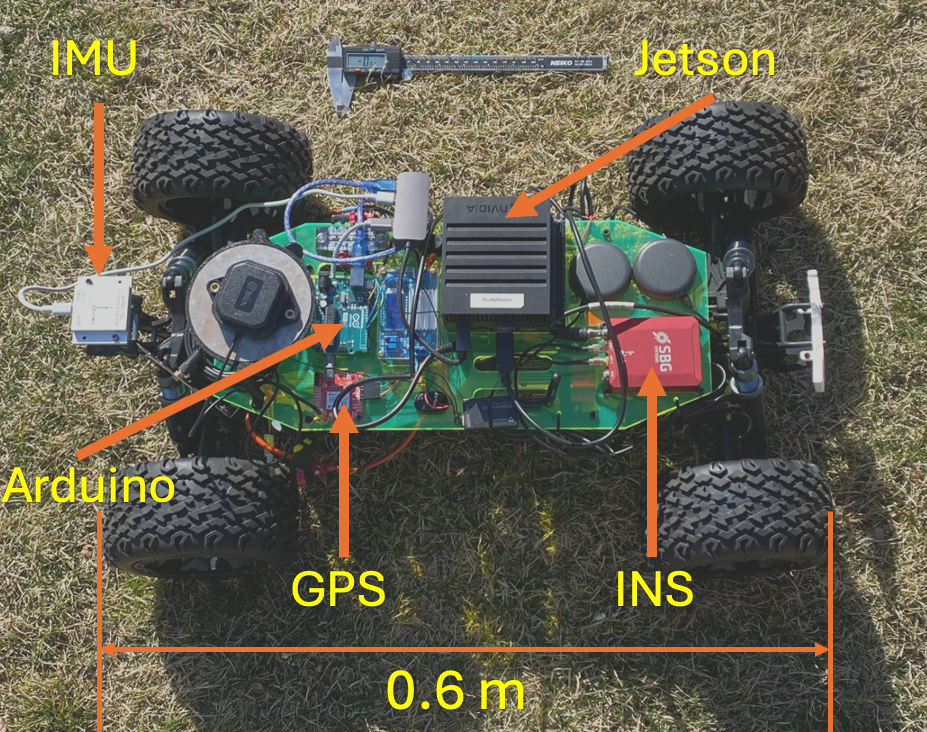
\includegraphics[width=\linewidth]{./images/art.png}
    \caption{ART Vehicle with all the available sensors}
    \label{fig:art}
  \end{subfigure}
  \hfill
  \begin{subfigure}[b]{0.45\textwidth}
    \centering
    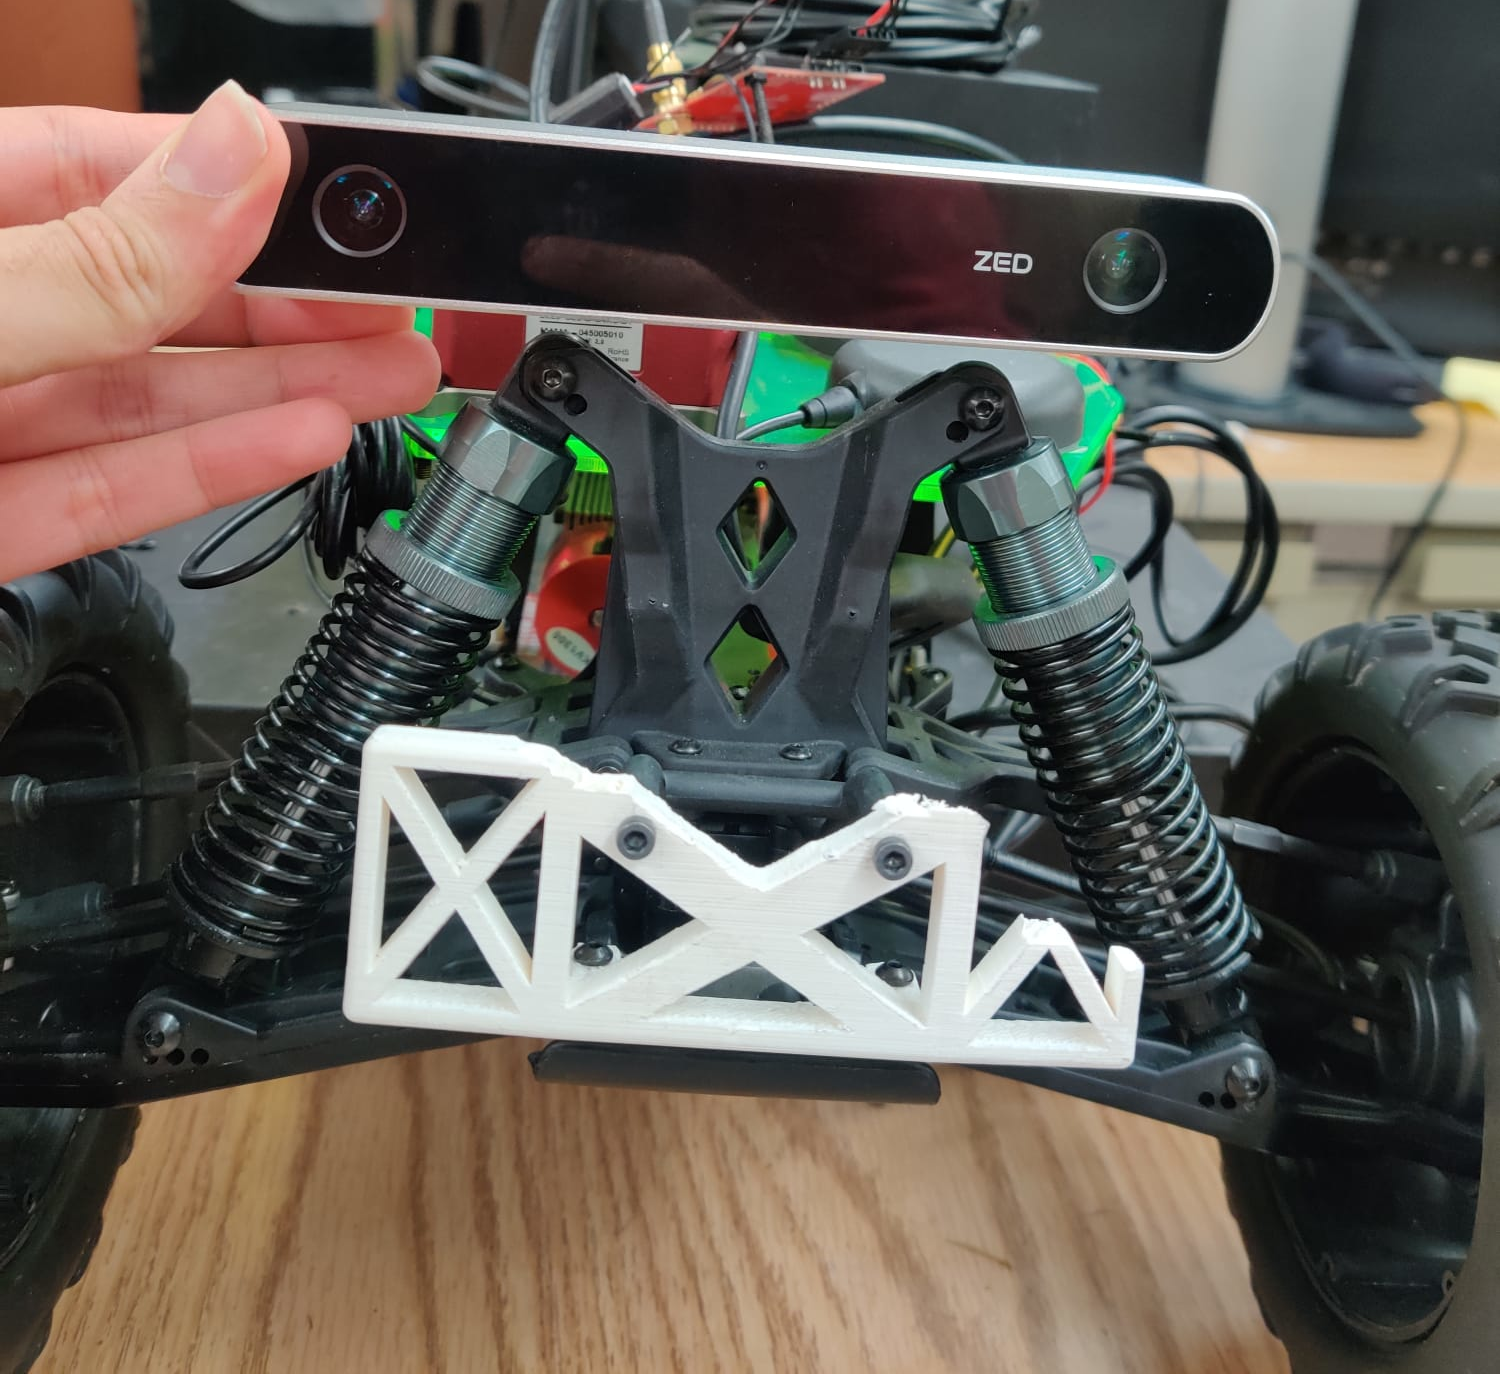
\includegraphics[width=\linewidth]{./images/camera.png}
    \caption{Camera with its potential position on ART (mount is getting 3D printed)}
    \label{fig:zed_2}
  \end{subfigure}
  \caption{ART along with the ZED 2 Stereo Camera}
  \label{fig:figure}
\end{figure}

\subsection{Simulation Environment Setup}
We utilize Project Chrono to establish a simulation environment that closely replicates the real-world vehicle. A 3D mesh of the ME3038 room and the \textit{ART} vehicle is constructed in Blender and imported for this purpose. This specific room is chosen due to its Motion Capture system, allowing us to validate the VO localization results obtained in the real world against ground truth localization offered by the motion capture system. Similarly, in simulation we can query the simulator for the ground truth vehicle position, providing us with all the ingredients to compute the localization error in both simulation and reality. We incorporate a stereo camera with parameters mirroring the actual ZED 2 camera. The figure below demonstrates a side-by-side comparison of the simulated and actual environments, including the camera outputs.

\begin{figure}[htbp]
    \centering
    \begin{subfigure}[b]{0.45\textwidth}
      \centering
      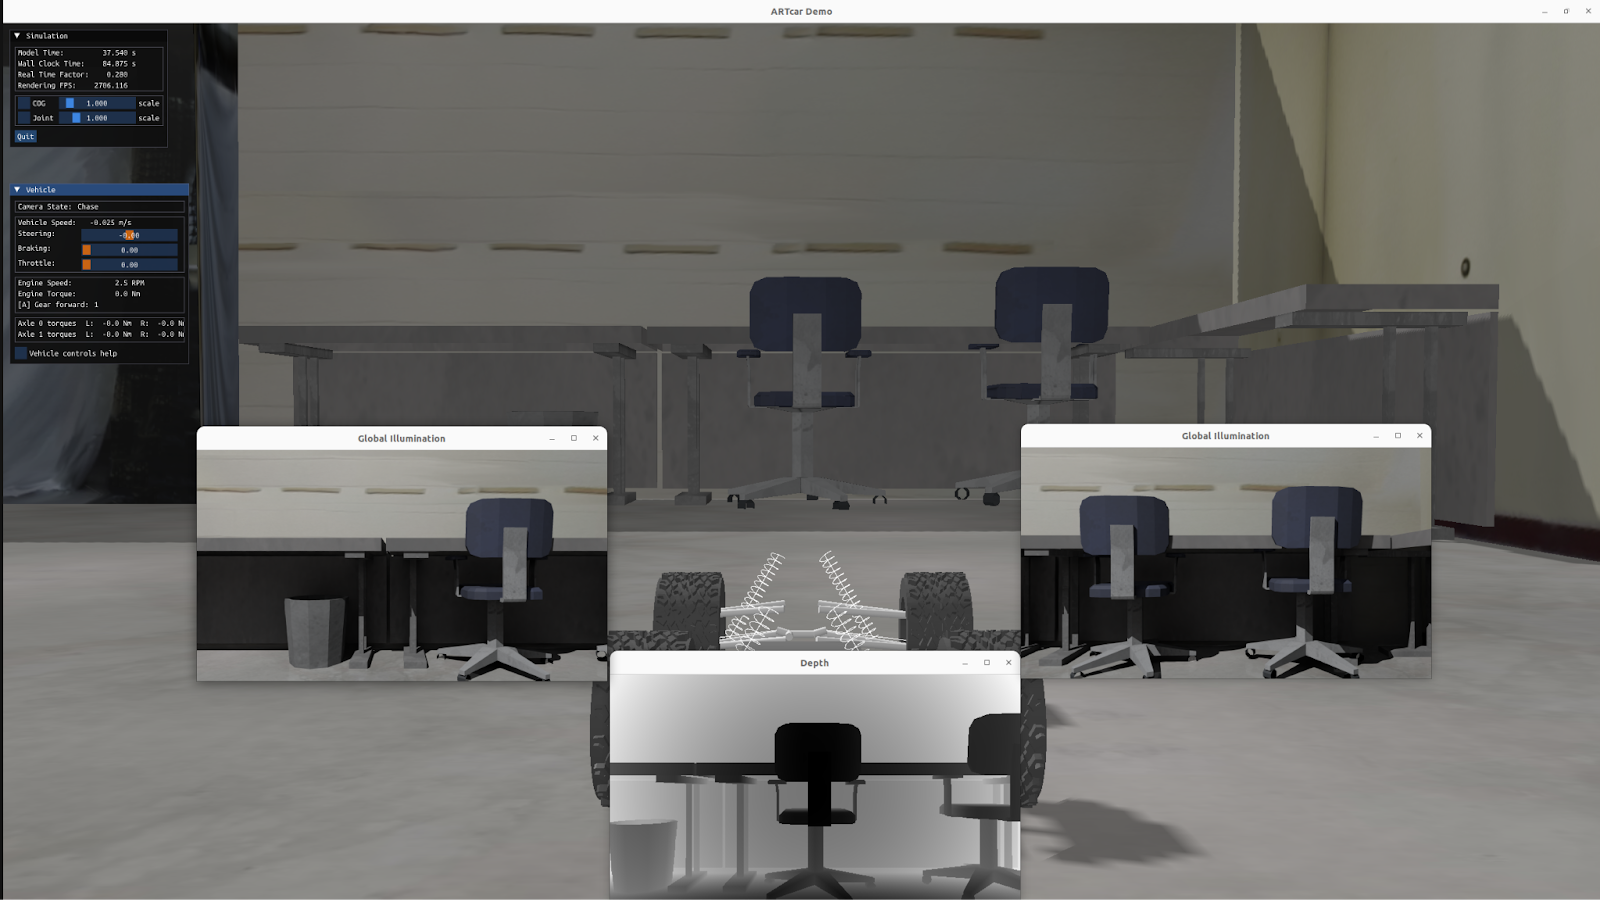
\includegraphics[width=\linewidth]{./images/sim.png}
      \caption{ART Vehicle in simulated environment with Stereo camera feed and depth map}
      \label{fig:sim}
    \end{subfigure}
    \hfill
    \begin{subfigure}[b]{0.45\textwidth}
      \centering
      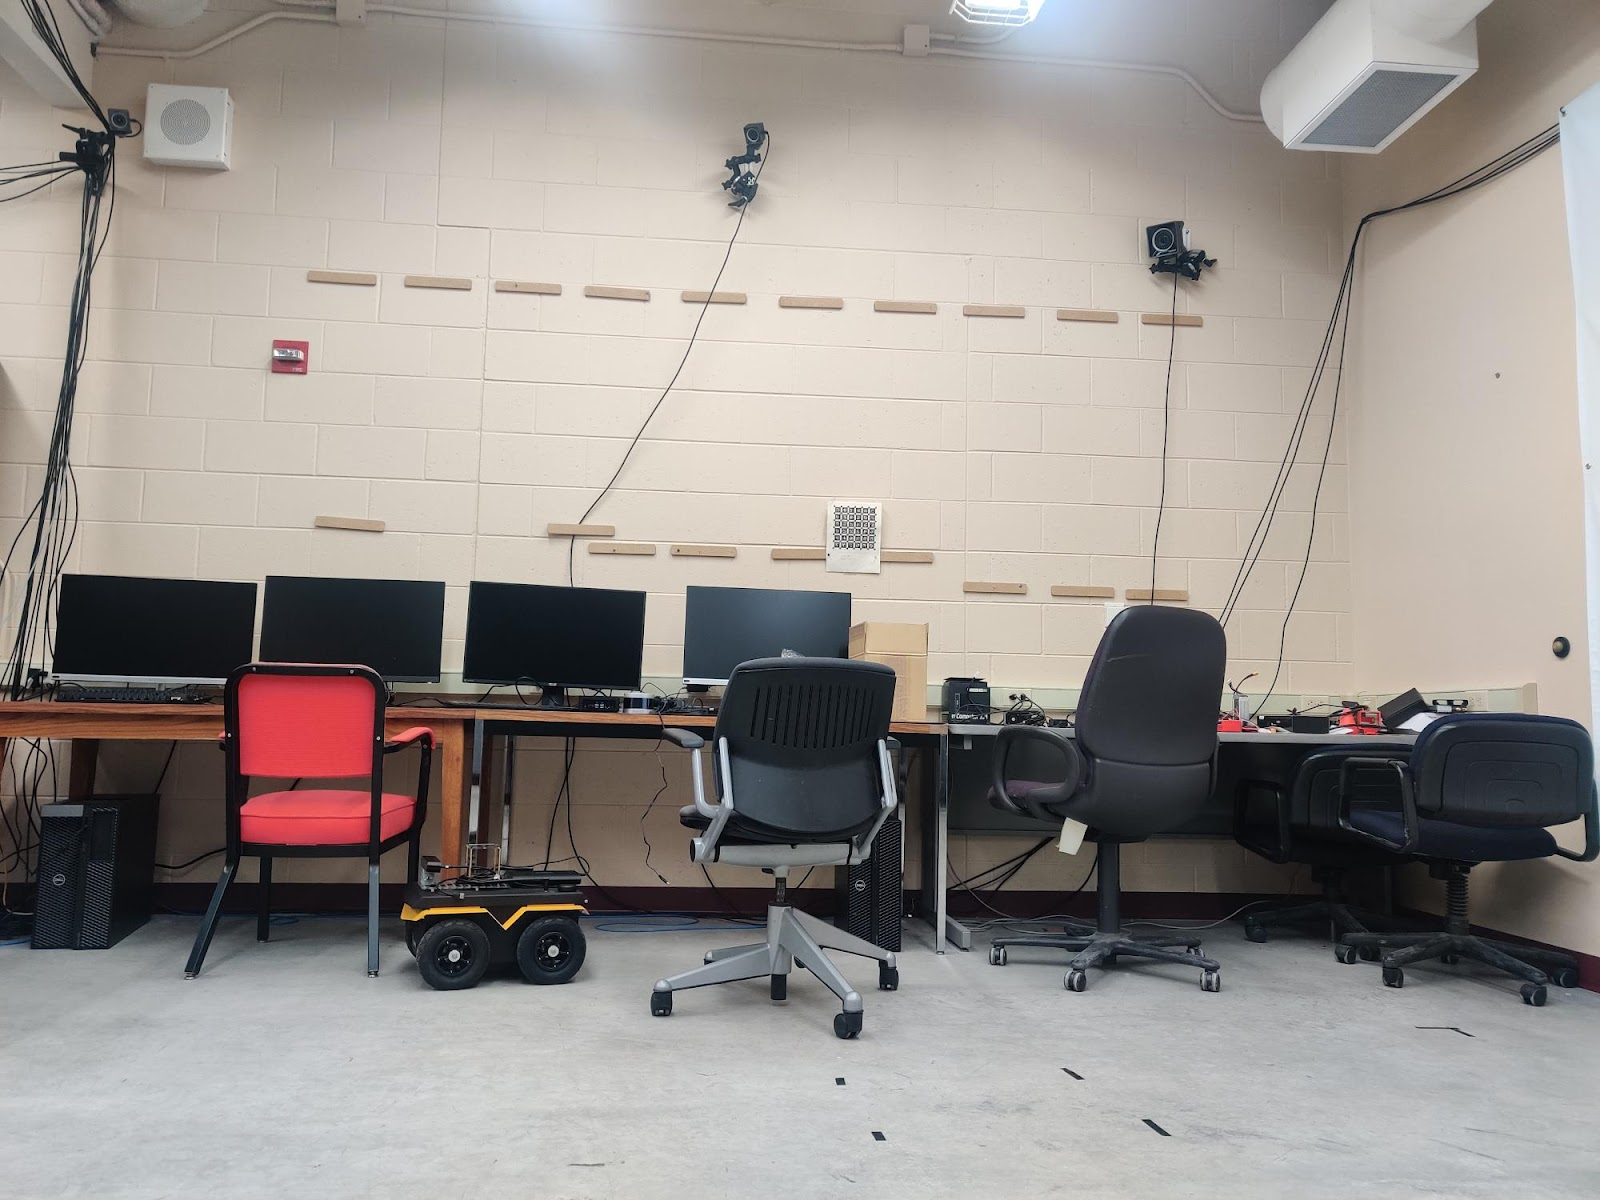
\includegraphics[width=\linewidth]{./images/real.jpeg}
      \caption{Picture taken in the real ME3808 room}
      \label{fig:real}
    \end{subfigure}
    \caption{Simulation and real environments}
    \label{fig:sim2real}
  \end{figure}

\href{https://uwmadison.box.com/s/6fg0vdrrqs0u74fcvunobefagvzrdkbu}{Here} is also a video of us driving ART in the simulated environment. As it can be seen, there is still a difference in the lighting and the actual features (computers, colors of chairs etc.). These are bound to change and cannot be exactly reproduced by a mesh generated manually. In future work, we detail methods in which we hope to create a more accurate mesh. 
% Use \includegraphics for images, e.g., \includegraphics[width=\linewidth]{path/to/your/image.jpg}


\section{Initial Results}
Due to a variety of bugs, here we only present preliminary findings based on tests with AirVO and Kimera-VIO algorithms. The purpose of this is to provide a sanity check to ensure that we are able to run these algorithms and extract results from them. 
\subsubsection*{AirVO}
The graph shows the output trajectory after running the algorithm on the UMA Visual-Inertial Dataset which was used by the authors of the paper. This dataset uses the images and imu data generated from a drone flying through a classroom. This was also generated using the ROS1 wrapper of the algorithm The arrows represent the orientation of the drone and the blue line is the estimated trajectory.

\begin{figure}[htbp]
    \centering
    \begin{subfigure}[b]{0.45\textwidth}
      \centering
      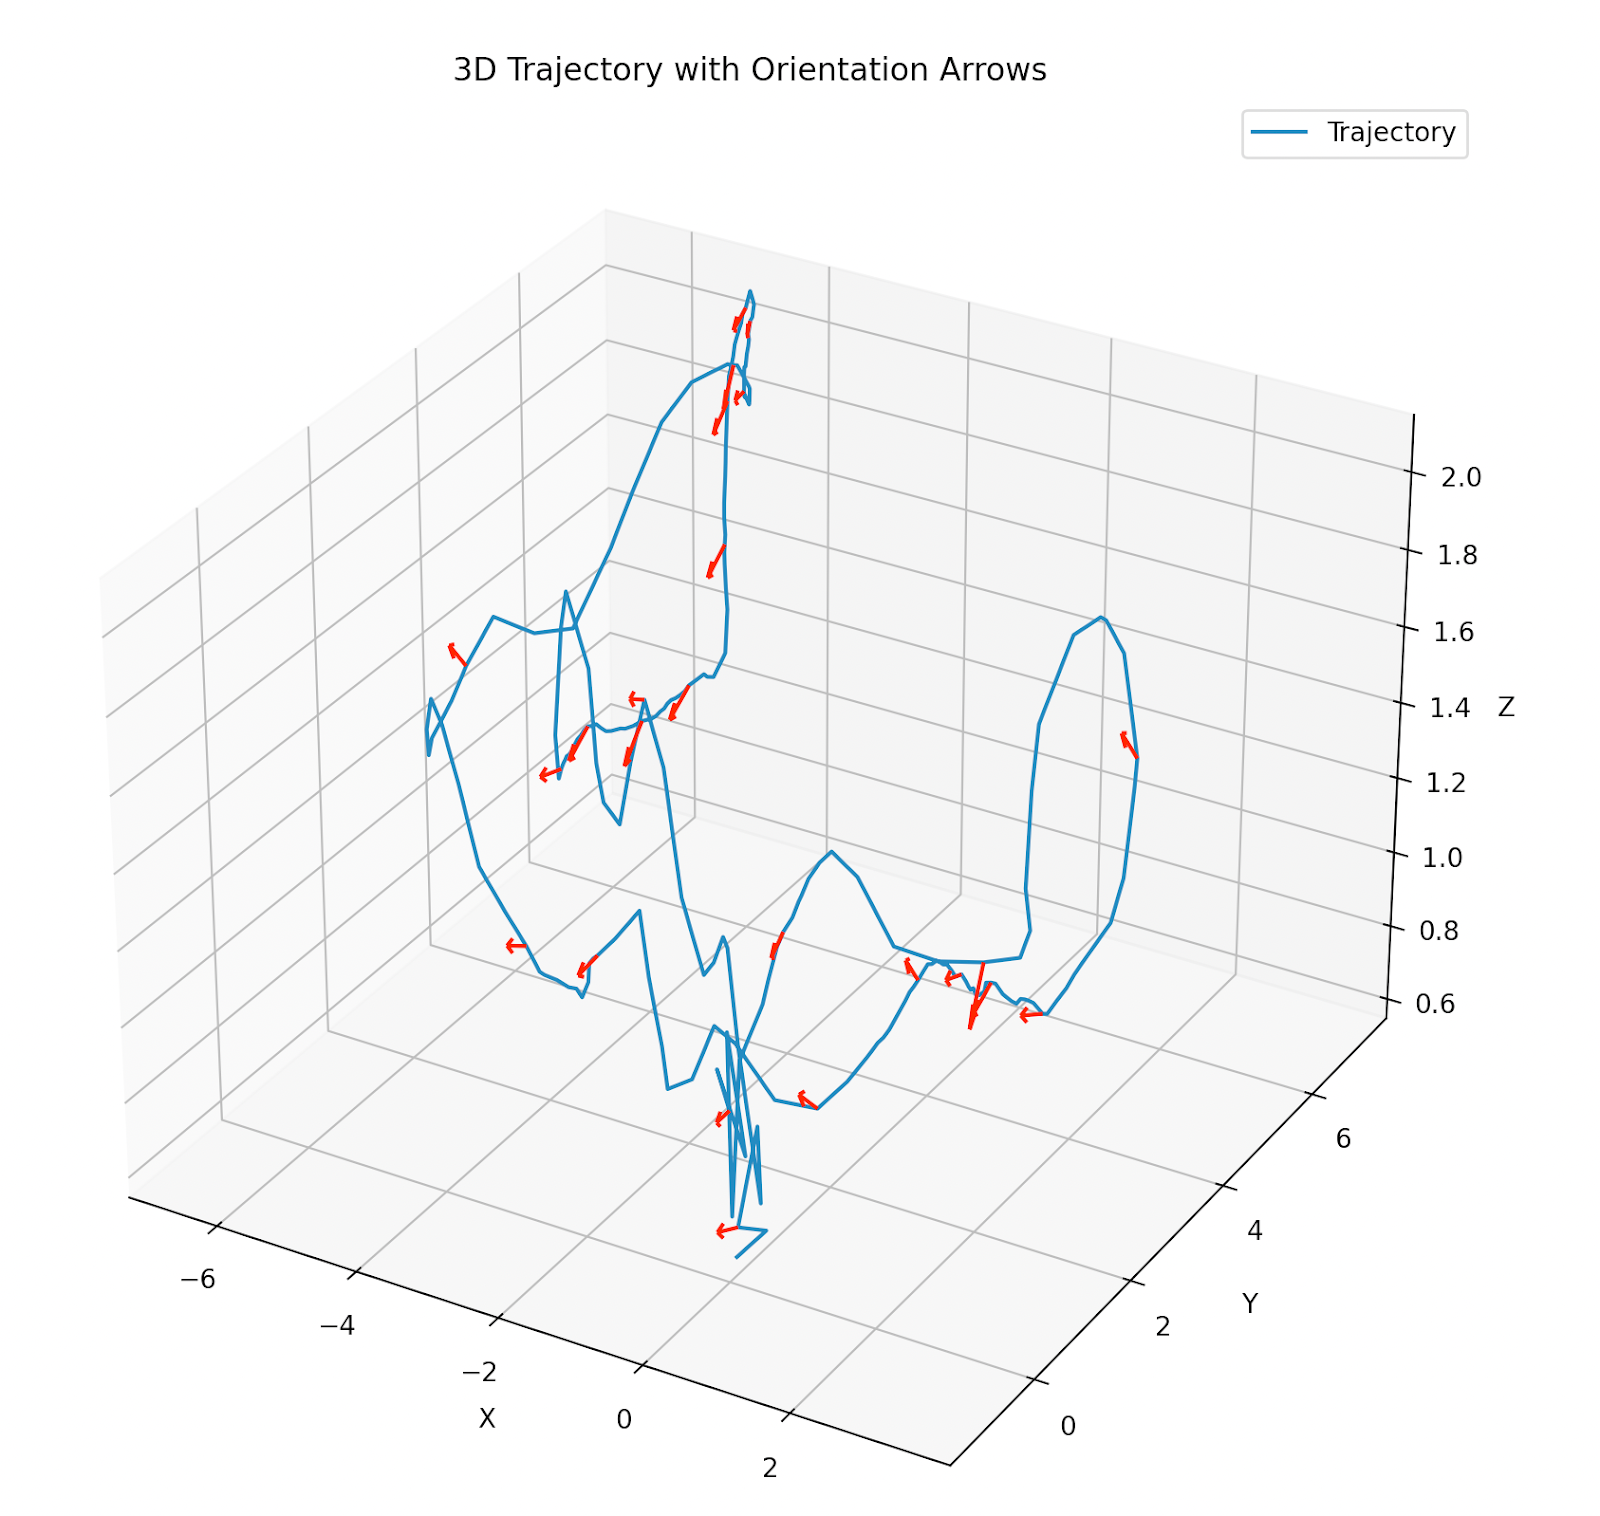
\includegraphics[width=\linewidth]{./images/airvo1.png}
      \caption{ADD CAPTION}
      \label{fig:airvo1}
    \end{subfigure}
    \hfill
    \begin{subfigure}[b]{0.45\textwidth}
      \centering
      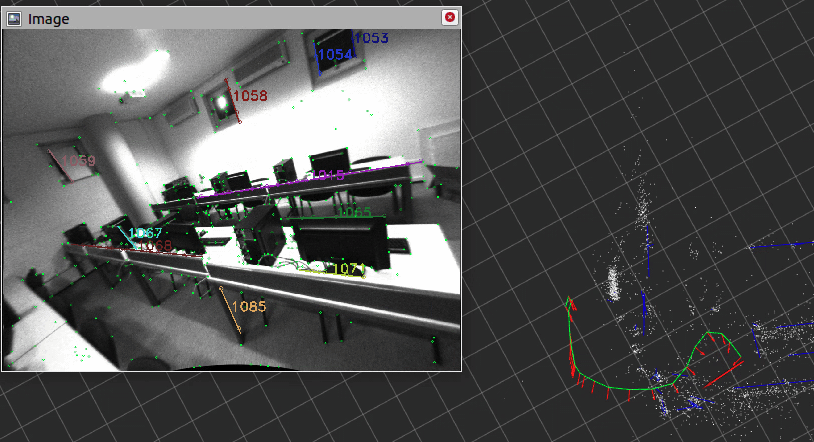
\includegraphics[width=\linewidth]{./images/airvo2.png}
      \caption{ADD CAPTION}
      \label{fig:airvo2}
    \end{subfigure}
    \caption{ADD CAPTION}
    \label{fig:airvo}
  \end{figure}

\subsubsection*{Kimera VIO}
We executed the Kimera-VIO algorithm on a sample EUROC dataset – specifically, the Vicon Room 2 01, which was also collected via drone (see here for more details). A \href{https://uwmadison.box.com/s/6fg0vdrrqs0u74fcvunobefagvzrdkbu}{video} of the run is available here. The results suggest that the Kimera-VIO algorithm functions effectively.

\section{Planned Project Activities}
Having most of the pieces in place, the future tasks are as follows
\begin{enumerate}
    \item Complete setup of ORB\_SLAM3 and VINS-Fusion. Each of these algorithms are close to set up and should not be far away from being ready. 
    \item Implement each of the algorithms into the existing ROS2 stack and conduct experiments in the simulation set-up. This will involve adding a node for each of the algorithms in the ROS2 stack.
    \item Use the same stack on the real vehicle with ZED 2. This involves mounting ZED 2 onto the vehicle (mount being 3D printed) and then setting up the autonomy stack and its dependencies on the compute - an Nvidia Jetson AGX.
    \item Obtaining data, coming up with a mathematical metric and evaluating the sim2real gap. Although we do not expect to complete many tests, this setup will be used in the lab internally to complete a robust evaluation of the sim2real gap.
\end{enumerate}

\section{Member contributions}
All members contributed equally to the various components of the project.

\end{document}